\section{Appendix}

\subsection{Documents and Code}
In addition to the thesis document, python code is also part of this master's thesis.
The main library is the \textit{TimeSeriesModelCreator\_Parallel\_talos.py} file. This can be used to create LSTM prediction models.

Examples of the usage of the library can be found in the experiment files. An example is experiment one.

\begin{scriptsize}
\begin{lstlisting}
#!/usr/bin/env python

from TimeSeriesModelCreator_Parallel_talos import
	TimeSeriesModelCreator_Parallel_talos
import pandas as pd
import matplotlib.pyplot as plt

look_backs = [1]
modelCreators = []
for look_back in look_backs:
	modelCreators.append(TimeSeriesModelCreator_Parallel_talos
	(look_back,
	r'..\Datasets\GEANTCombined\all_in_one_complete_appended.csv'))

for modelCreator in modelCreators:
	batch_sizes = [100]
	epochs = [100,250,500,750,1000]
	nodes = [1, 2, 3, 8, 16, 32, 64, 128]
	layers = [1]
	optimizers = ['adam']
	losses = ['mean_squared_error']
	modelCreator.test_for_optimal_config('Epxeriment_1_1', 1, 5, 11, 11,
		1000, batch_sizes, epochs, nodes, layers, optimizers, losses,
		40,	1, 0, 200)
\end{lstlisting}
\end{scriptsize}

This is an example for testing multiple parameter variations.
From the results of this optimization a model can be created and the model is saved in the library object. Where it can be called using its name.
An example for this can be found in the Jupyter notebooks comparing the LSTM and the ARIMA models.
The following example creates five different models and uses them to predict traffic.

\begin{samepage}
\begin{scriptsize}
	\begin{lstlisting}
creator = TimeSeriesModelCreator_Parallel_talos(2,
	r'..\Datasets\GEANTCombined\all_in_one_complete_appended.csv')
modelMatch = {}
for x in range(1,6):
	creator.add_new_model(name = 'test'+str(x), nodes = 1, layer = 1, 
		loss='mean_squared_error', optimizer='adam')
	modelMatch[str(x)+'_11'] = 'test'+str(x)
	creator.train_model(1, 5, 11, 11, 1000, 200, modelMatch, 
		epoch = 1000, batch_size = 128, shift = 0)
	
LSTMpredictions = []
for x in range(1,6):
	prediction = creator.predict('test'+str(x), subsets_testing[x-1], 0)
	LSTMpredictions.append(prediction)
	\end{lstlisting}
\end{scriptsize}
\end{samepage}

These two examples cover most of the functionallities of the library. 
More examples and the library itself can be found in the \textit{source/Training} folder.

\subsection{Libraries and Frameworks}
\begin{itemize}
	\item Python 3.6.1
	\item Keras 2.2.5
	\item TensorFlow 1.14.0
	\item Talos 0.6.3
	\item Pandas 0.24.2
	\item sklearn 0.21.3
\end{itemize}

\subsection{Figures}
   
	\begin{figure}[H]
		\centering
		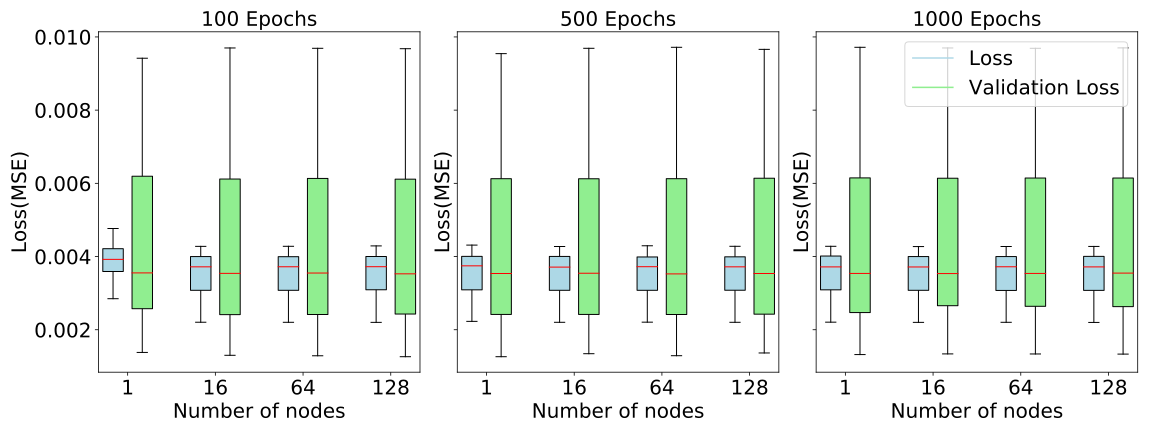
\includegraphics[width=1\linewidth]{Pictures/Results/experiment_1_1_2}
		\caption{The loss and validation loss when increasing the number of hidden nodes. Pair (2, 11)}
		\label{fig:experiment_1_1_2}
	\end{figure}
	\begin{figure}[H]
		\centering
		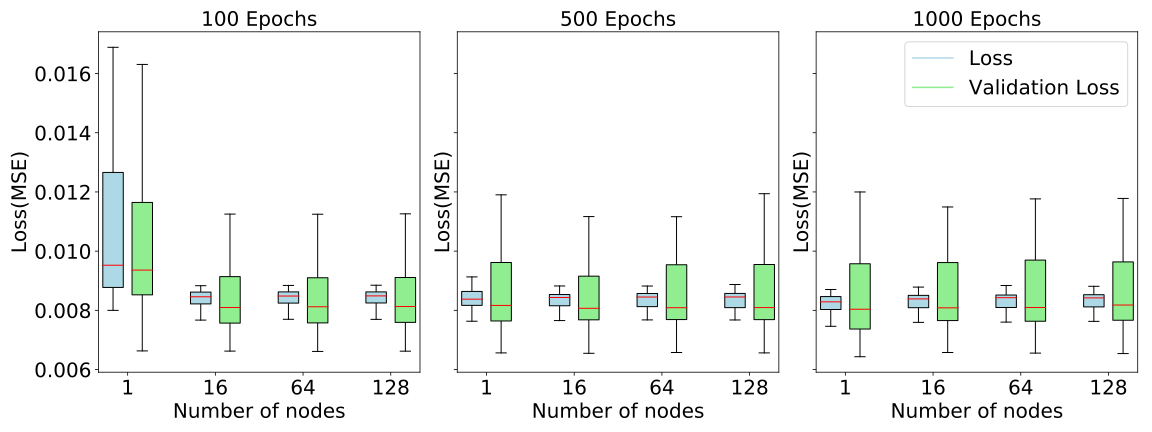
\includegraphics[width=1\linewidth]{Pictures/Results/experiment_1_1_3}
		\caption{The loss and validation loss when increasing the number of hidden nodes. Pair (3, 11)}
		\label{fig:experiment_1_1_3}
	\end{figure}
	\begin{figure}[H]
		\centering
		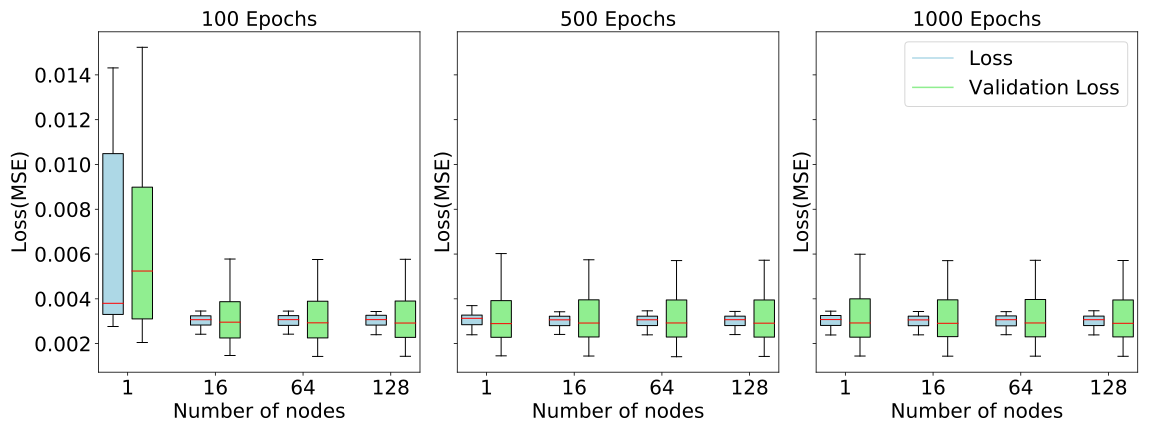
\includegraphics[width=1\linewidth]{Pictures/Results/experiment_1_1_4}
		\caption{The loss and validation loss when increasing the number of hidden nodes. Pair (4, 11)}
		\label{fig:experiment_1_1_4}
	\end{figure}
	\begin{figure}[H]
		\centering
		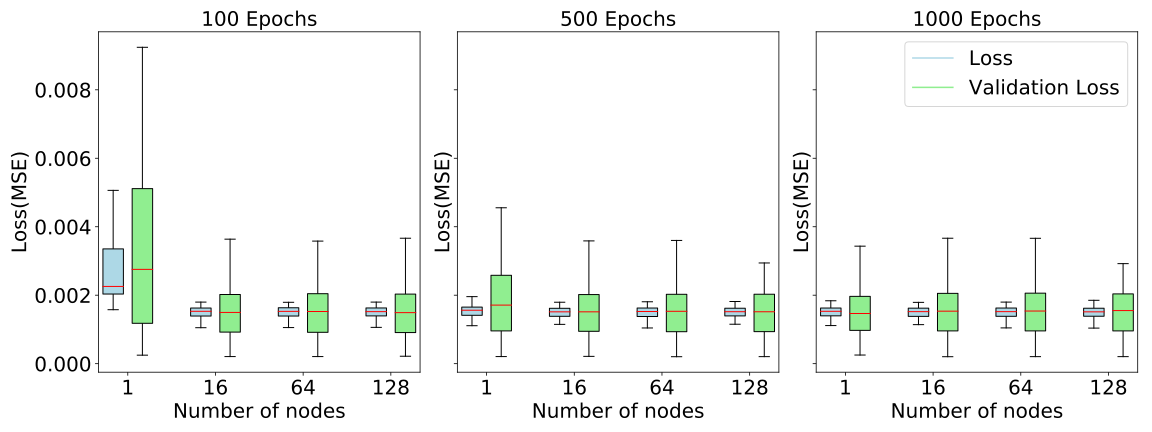
\includegraphics[width=1\linewidth]{Pictures/Results/experiment_1_1_5}
		\caption{The loss and validation loss when increasing the number of hidden nodes. Pair (5, 11)}
		\label{fig:experiment_1_1_5}
	\end{figure}


	\begin{figure}[H]
		\centering
		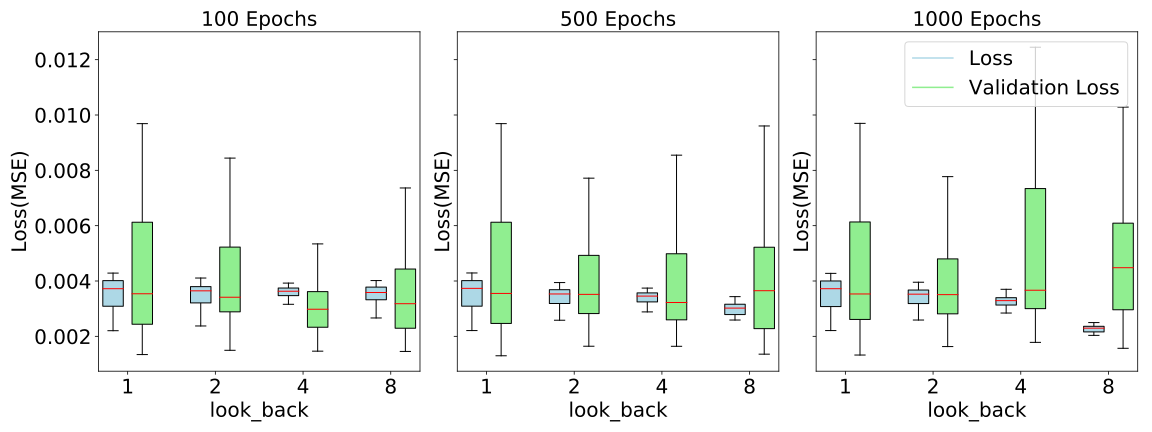
\includegraphics[width=1\linewidth]{Pictures/Results/experiment_2_1_2}
		\caption{The loss and validation loss when increasing the number of previous values to take into account for a prediction. Pair (2, 11)}
		\label{fig:experiment_2_1_2}
	\end{figure}
	\begin{figure}[H]
		\centering
		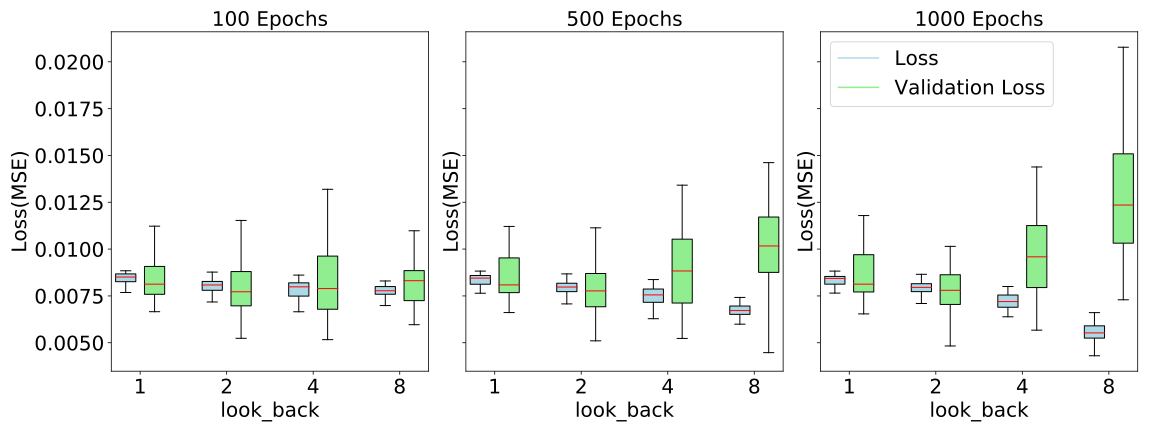
\includegraphics[width=1\linewidth]{Pictures/Results/experiment_2_1_3}
		\caption{The loss and validation loss when increasing the number of previous values to take into account for a prediction. Pair (3, 11)}
		\label{fig:experiment_2_1_3}
	\end{figure}
	\begin{figure}[H]
		\centering
		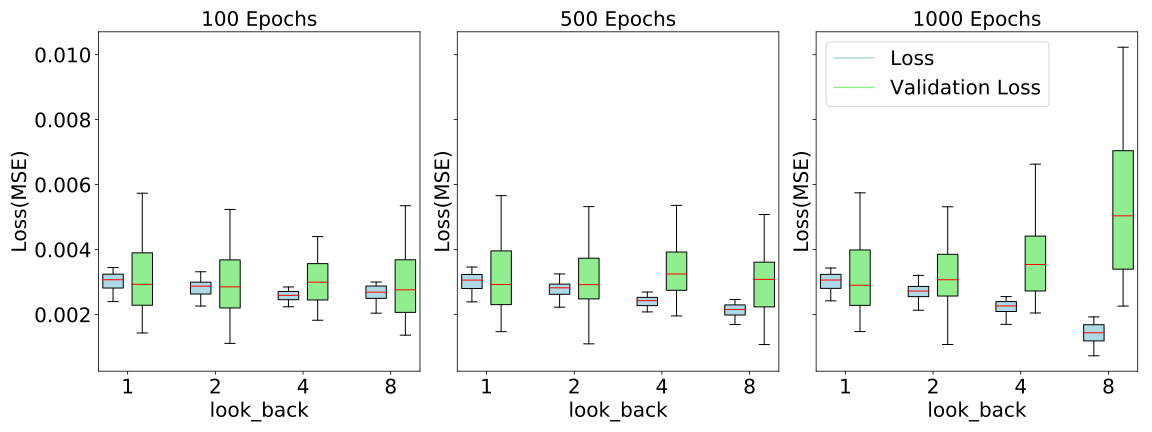
\includegraphics[width=1\linewidth]{Pictures/Results/experiment_2_1_4}
		\caption{The loss and validation loss when increasing the number of previous values to take into account for a prediction. Pair (4, 11)}
		\label{fig:experiment_2_1_4}
	\end{figure}
	\begin{figure}[H]
		\centering
		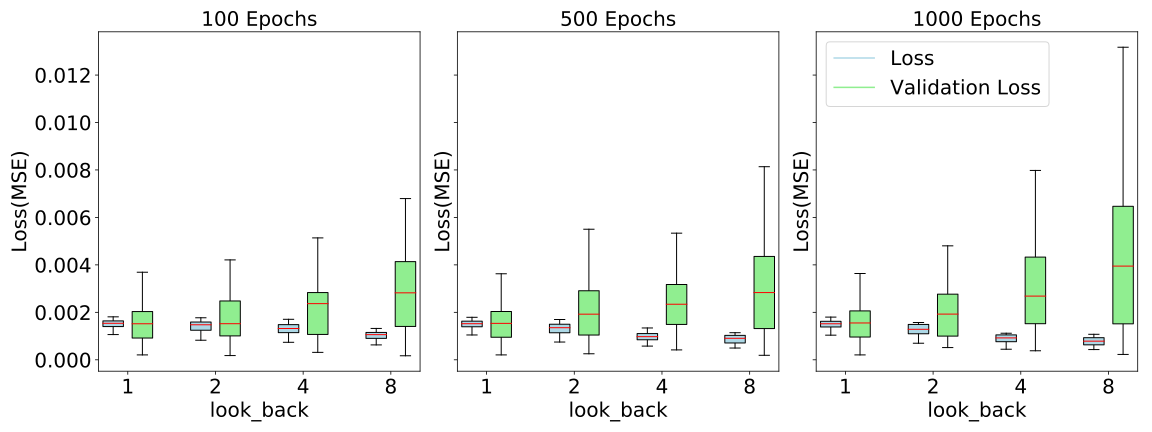
\includegraphics[width=1\linewidth]{Pictures/Results/experiment_2_1_5}
		\caption{The loss and validation loss when increasing the number of previous values to take into account for a prediction. Pair (5, 11)}
		\label{fig:experiment_2_1_5}
	\end{figure}


	\begin{figure}[H]
		\centering
		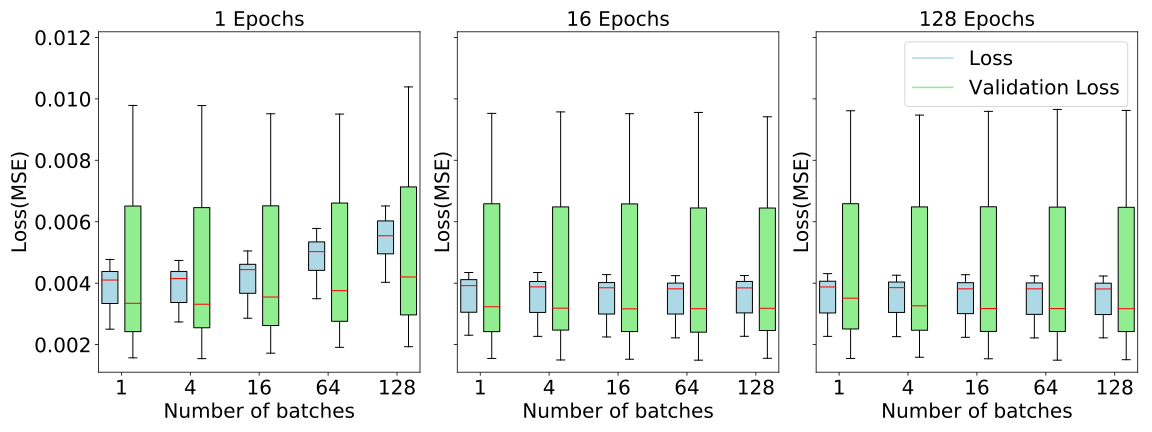
\includegraphics[width=1\linewidth]{Pictures/Results/experiment_4_2}
		\caption{The impact of epochs vs. number of batches. Pair (2, 11)}
		\label{fig:experiment_4_2}
	\end{figure}
	\begin{figure}[H]
		\centering
		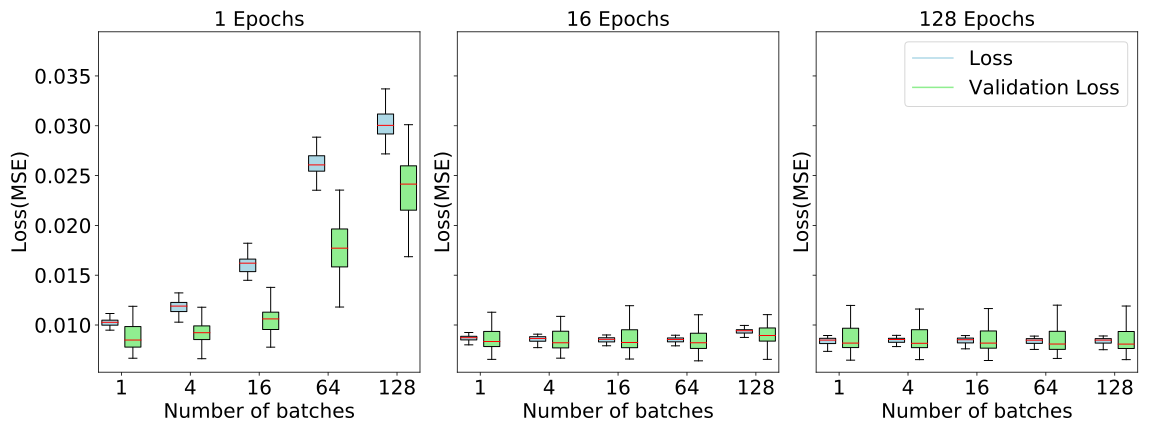
\includegraphics[width=1\linewidth]{Pictures/Results/experiment_4_3}
		\caption{The impact of epochs vs. number of batches. Pair (3, 11)}
		\label{fig:experiment_4_3}
	\end{figure}
	\begin{figure}[H]
		\centering
		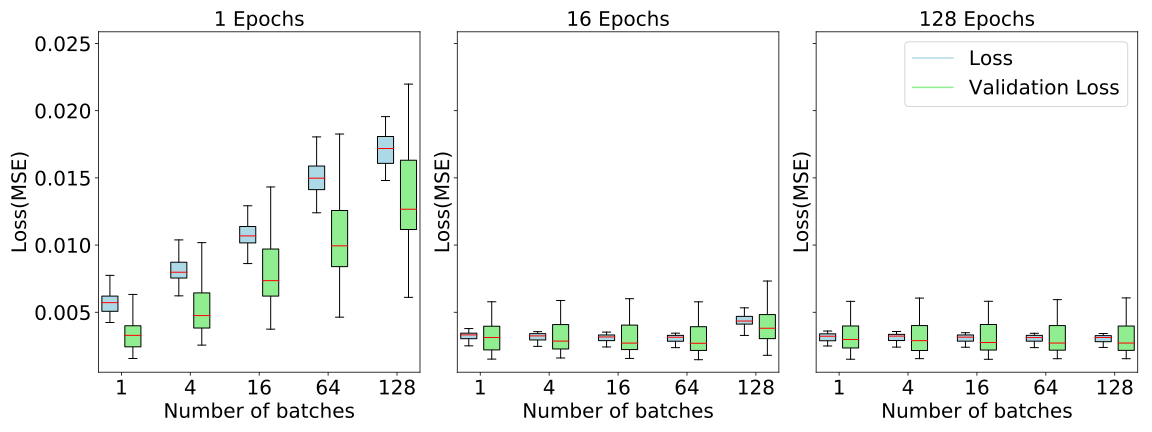
\includegraphics[width=1\linewidth]{Pictures/Results/experiment_4_4}
		\caption{The impact of epochs vs. number of batches. Pair (4, 11)}
		\label{fig:experiment_4_4}
	\end{figure}
	\begin{figure}[H]
		\centering
		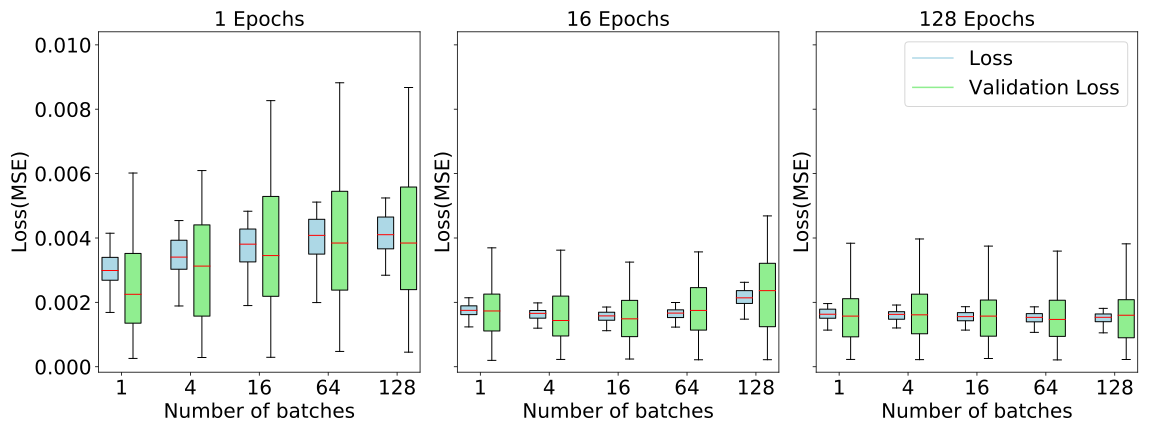
\includegraphics[width=1\linewidth]{Pictures/Results/experiment_4_5}
		\caption{The impact of epochs vs. number of batches. Pair (5, 11)}
		\label{fig:experiment_4_5}
	\end{figure}


	\begin{figure}[H]
		\centering
		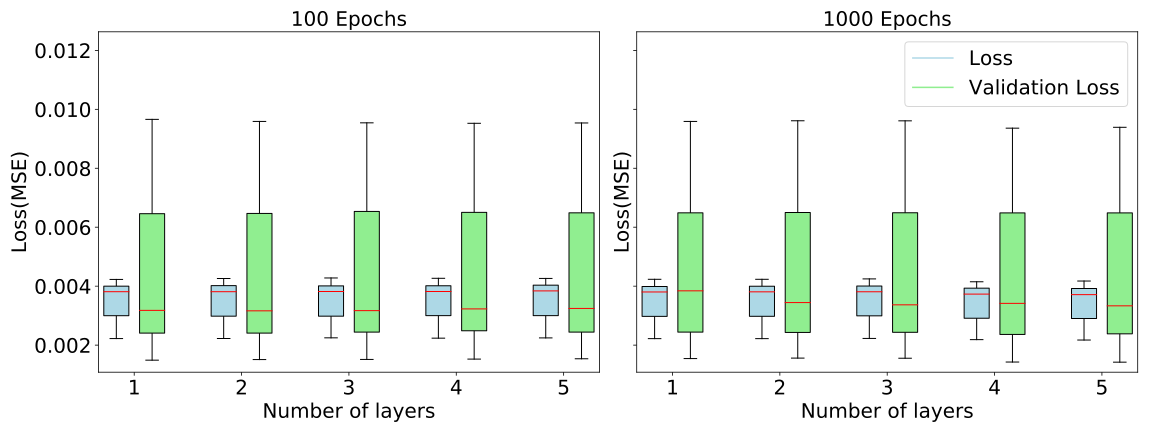
\includegraphics[width=1\linewidth]{Pictures/Results/experiment_3_2}
		\caption{Plot of how the number of LSTM layers influence the loss and validation loss. Pair (2, 11)}
		\label{fig:experiment_3_2}
	\end{figure}
	\begin{figure}[H]
		\centering
		\includegraphics[width=1\linewidth]{Pictures/Results/experiment_3_3}
		\caption{Plot of how the number of LSTM layers influence the loss and validation loss. Pair (3, 11)}
		\label{fig:experiment_3_3}
	\end{figure}
	\begin{figure}[H]
		\centering
		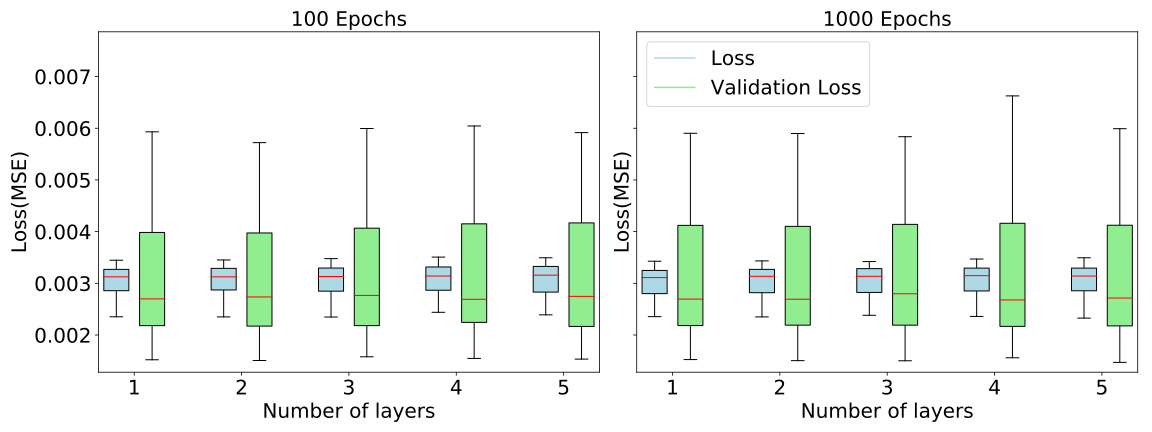
\includegraphics[width=1\linewidth]{Pictures/Results/experiment_3_4}
		\caption{Plot of how the number of LSTM layers influence the loss and validation loss. Pair (4, 11)}
		\label{fig:experiment_3_4}
	\end{figure}
	\begin{figure}[H]
		\centering
		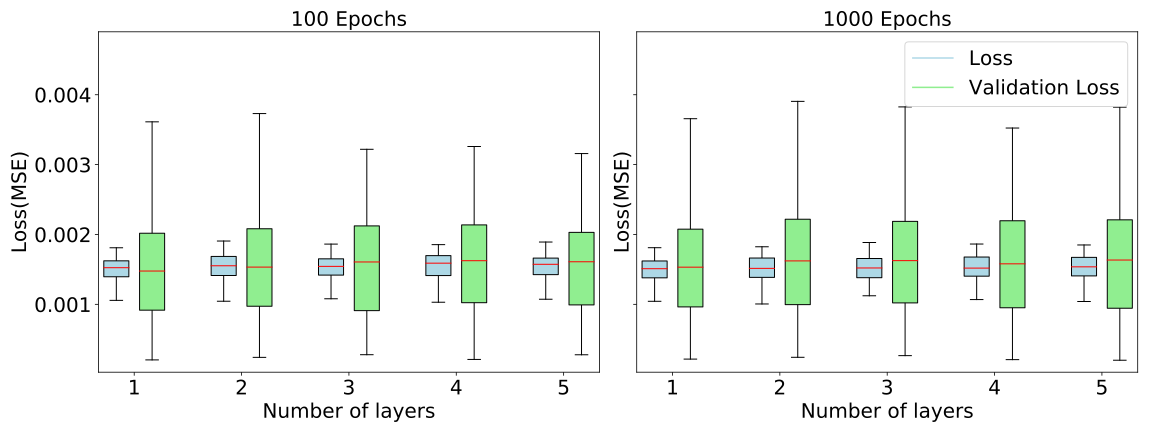
\includegraphics[width=1\linewidth]{Pictures/Results/experiment_3_5}
		\caption{Plot of how the number of LSTM layers influence the loss and validation loss. Pair (5, 11)}
		\label{fig:experiment_3_5}
	\end{figure}


	\begin{figure}[H]
		\centering
		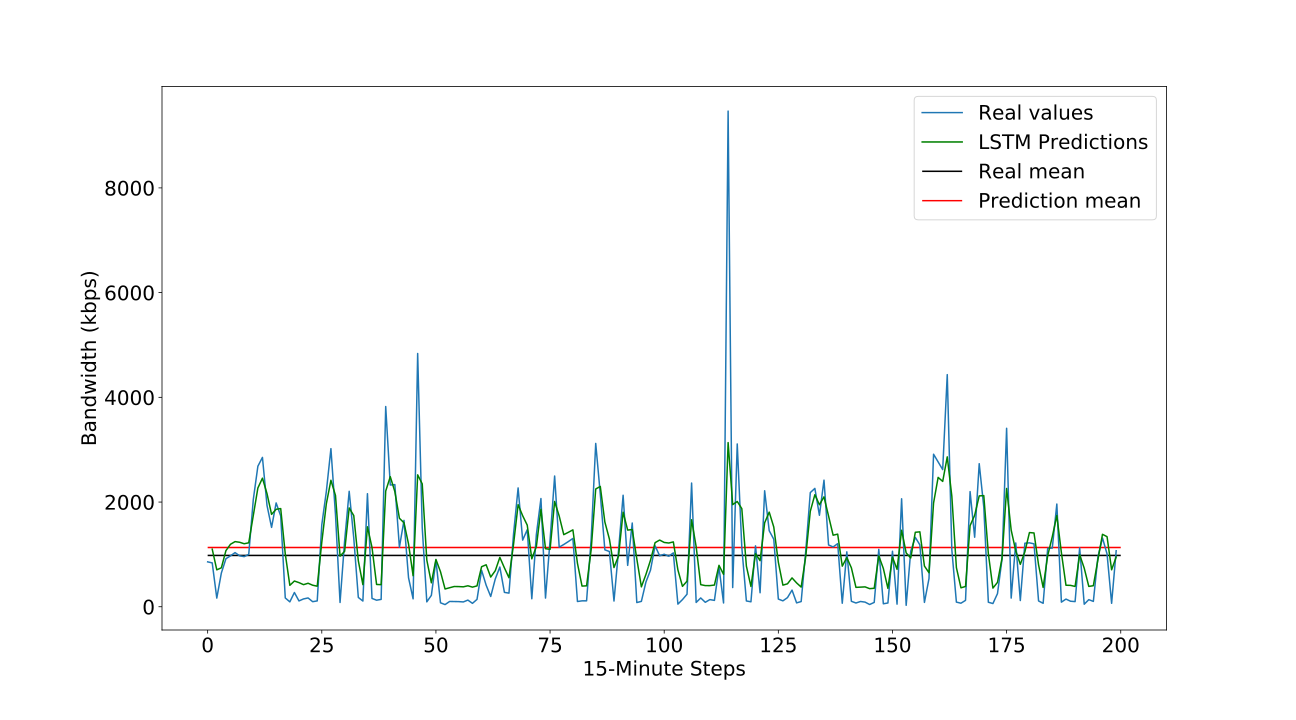
\includegraphics[width=1\linewidth]{Pictures/Practical_Examples/LSTMprediction_0}
		\caption{LSTM prediction of pair (1, 11)}
		\label{fig:LSTMprediction_0}
	\end{figure}
	\begin{figure}[H]
		\centering
		\includegraphics[width=1\linewidth]{Pictures/Practical_Examples/LSTMprediction_2}
		\caption{LSTM prediction of pair (3, 11)}
		\label{fig:LSTMprediction_2}
	\end{figure}
	\begin{figure}[H]
		\centering
		\includegraphics[width=1\linewidth]{Pictures/Practical_Examples/LSTMprediction_4}
		\caption{LSTM prediction of pair (5, 11)}
		\label{fig:LSTMprediction_4}
	\end{figure}


\begin{figure}[H]
		\centering
		\includegraphics[width=1\linewidth]{Pictures/Practical_Examples/AvLprediction_0}
		\caption{LSTM and ARIMA predictions of pair (1, 11)}
		\label{fig:ARIMAprediction_0}
\end{figure}
\begin{figure}[H]
		\centering
		\includegraphics[width=1\linewidth]{Pictures/Practical_Examples/AvLprediction_2}
		\caption{LSTM and ARIMA predictions of pair (3, 11)}
		\label{fig:ARIMAprediction_2}
\end{figure}
\begin{figure}[H]
		\centering
		\includegraphics[width=1\linewidth]{Pictures/Practical_Examples/AvLprediction_3}
		\caption{LSTM and ARIMA predictions of pair (4, 11)}
		\label{fig:ARIMAprediction_3}
\end{figure}